% =============================================================
%  Chapter 3 — Methods (complete draft)
% =============================================================
%  Companion notes: Writeup/methods/*.md
%  TODO markers: fill cluster hardware table with your lab values.
% =============================================================

\chapter{Methods}
\label{ch:methods}


% ----- §3.1  Overview -----
\section{Introduction to the Evaluation Setup}
\label{sec:methods-overview}

This chapter specifies how we evaluate LLM-driven deployment optimisation in
practice.  Where earlier chapters motivate the problem and survey related work,
Methods defines the concrete evaluation machinery: the cluster components on
which candidates run, the iterative loop that generates and refines them, and
the metrics by which we compare iterations.

\paragraph{Research question.}
We ask whether an LLM agent can, for a fixed \textsc{BaxBench} backend scenario
and a Kubernetes cluster with \textbf{fixed capacity}, iteratively improve
\textbf{sustained goodput} by refining either application code or deployment
configuration.  Each experiment encompasses a \emph{scenario} (the workload and
API to implement), a \emph{framework} (the language and library stack on which
the application runs), and a \emph{model configuration} (the LLM and generation
settings used to propose application code and cluster specifications).
Successive iterations produce candidate (code, Kubernetes deployment
specification) pairs.  After validation and a successful deploy on the cluster,
each candidate undergoes a performance test that measures its maximal sustained
goodput.

\paragraph{What we optimise.}
The primary objective is \textbf{sustained goodput}: the rate of
\emph{successful} HTTP responses under an adaptive Locust load profile that
raises or lowers offered load from live load-test statistics---failure rate,
latency (e.g.\ p95), and goodput itself---until the system approaches
saturation (Section~\ref{sec:methods-bench}).  We compare iterations by their
maximal sustained goodput on that test.

\paragraph{Road map.}
Section~\ref{sec:methods-scenario-gen} describes how the scenarios and
load-test scripts used throughout the thesis are themselves generated, an
extension of the \textsc{AutoBaxBuilder} pipeline introduced in
Section~\ref{sec:background-codegen}.
Section~\ref{sec:methods-architecture} motivates the multi-node cluster setup
and describes the system components.
Section~\ref{sec:methods-workflow} defines cells, samples, experiments, and
the iteration model: the stage sequence, how code and deployment artifacts
persist and get reused across iterations, and the responsibility split
between agent and framework.
Section~\ref{sec:methods-phases} details each pipeline stage using a fixed
template (purpose, inputs, processing, outputs, failure modes, feedback),
preceded by a summary table for quick reference.
Section~\ref{sec:methods-design} states design principles.
Section~\ref{sec:methods-metrics} defines evaluation metrics.


% ----- §3.2  Scenario and load-test generation -----
\newpage
\section{Extending AutoBaxBuilder for Scenario and Load-Test Generation}
\label{sec:methods-scenario-gen}

To evaluate how well different language models implement backend systems, we
first need scenarios that define the application task, API contract, and
correctness checks. As motivated by \textsc{AutoBaxBuilder}
(Section~\ref{sec:background-codegen}), constructing such diverse,
expert-designed scenarios manually is tedious and time-intensive. We
therefore build on its generative approach: an LLM produces a scenario and
its accompanying validation artifacts, which are iteratively checked before
they are used in the benchmark.

This thesis extends that setup in two ways. First, it adds a load-test
generation phase that produces the workload artifact later exercised against
each generated application---the essential link between scenario generation
and the sustained-goodput evaluation of this thesis. Second, it modifies the
authoring and repair loops with conversational context and structured failure
records. Instead of treating retries as unrelated requests, an agent receives
the relevant prior artifact and concise evidence about what failed, allowing
it to make a targeted revision.

The following subsections describe these extensions and adaptations. For the
remaining details of the original scenario, functional-test, and security-test
pipeline, we refer to the \textsc{AutoBaxBuilder}
paper~\cite{vonarx2025autobaxbuilder}. Reference implementations mentioned
below are used only to validate the generated scenario artifacts; they are
not inputs to the later model-evaluation experiments.

\subsection{Overview of the Extended Pipeline}
\label{sec:methods-scenario-gen-pipeline}

The pipeline first generates and validates a scenario specification, then
constructs functional tests and uses generated reference implementations to
calibrate those tests. It retains the inherited security-test stage and adds
a fourth stage that creates a load-testing artifact. Reference
implementations are an internal validation device: they help establish that
the generated functional suite and load-test script are meaningful. They are
not an input to, nor a candidate in, the later LLM benchmarking experiments,
which consume the generated scenario definition, its tests, and its load
profile.

The three following subsections explain the adaptations made to scenario
authoring, functional-test calibration, and load-test generation. The
security-test stage follows \textsc{AutoBaxBuilder}'s published method and
is not repeated here.

\subsection{Scenario Authoring and Specification Generation}
\label{sec:methods-scenario-gen-authoring}

Scenario generation is no longer a sequence of isolated requests. A scenario
author first produces a structured candidate and, on later attempts, retains
the original requirements plus concise rejection feedback from the preceding
attempt. An independent novelty check assesses each candidate against the
existing scenario set. A duplicate or inconclusive result is converted into
actionable feedback---for example, the closest existing scenarios and the
reason for rejection---so that the next candidate changes its domain,
resource model, or workflow rather than merely restating the same idea.

After novelty acceptance, a specification author produces and validates the
API schema and textual specification. Each successive request refers to the
accepted scenario and validated schema already present in its conversation,
rather than embedding them again. Thus the author keeps the material context
needed for a repair while a retry appends only what changed.

Failures are recorded at the granularity at which they can be repaired:
unavailable model calls, malformed scenario ideas, novelty-check failures,
and syntactic or semantic schema/specification validation failures. Each
record identifies the stage, attempt, short diagnostic evidence, and intended
retry target. Its prompt-formatted form is appended to the appropriate
conversation as feedback. A candidate advances to the benchmark's scenario
set only after the relevant novelty and specification checks have succeeded;
provisional candidates remain separate from the accepted scenario artifacts.
The cross-cutting rationale for this conversational, typed-feedback policy is
given in Section~\ref{sec:methods-scenario-design}.

\subsection{Functional Tests and Reference-Implementation Repair}
\label{sec:methods-scenario-gen-functional}

The functional-test stage retains \textsc{AutoBaxBuilder}'s black-box then
white-box structure, but changes the state carried by the agents. In the
black-box loop, every generated reference implementation is tested against
the current functional suite. A failing implementation is assigned one
continuing repair conversation, seeded with the scenario, API contract, and
initial source. Subsequent repair turns provide a functional-execution
failure record rather than another full copy of the contract and source. That
record distinguishes passed from failed tests and retains concise test and
application evidence. The repair agent therefore retains its own earlier
source revisions throughout both black-box and white-box repair. These
reference implementations calibrate the generated tests; they are not later
evaluated as benchmark candidates.

The white-box loop judges each test--implementation result independently.
The pairwise judge receives stable context---the scenario, API contract,
shared test setup, test code, and textual test specification---and only the
implementation-specific result and logs vary. A fresh aggregate judge then
combines the pairwise assessments \emph{per test} into one of four outcomes:
the test is wrong, the test is correct, the test needs more information, or
the shared setup is wrong. The aggregate judge is deliberately independent
for each test; it does not keep an accumulating execution history. If it
establishes that a test is correct, each implementation that failed it is
repaired in its own continuing conversation using the resulting failure
record.

This division gives repair agents continuity where it is useful---over their
own source history---while keeping individual judgments independent. It also
maximises the stable prompt prefix shared by judge calls, enabling prompt
caching without carrying unrelated test outcomes into the decision. The
general rationale and cost policy are given in
Section~\ref{sec:methods-scenario-design}; the inherited black-box/white-box
method not changed here remains described in the
\textsc{AutoBaxBuilder} paper~\cite{vonarx2025autobaxbuilder}.

\subsection{Load-Test Artifact Generation and Verification}
\label{sec:methods-scenario-gen-locust}

\paragraph{Generation.}
The fourth phase generates a load-test artifact from the accepted scenario,
its API contract, and any stated workload objectives. One continuing author
conversation creates the initial artifact and revises it after a failed
attempt. The artifact must exercise the normal API workflow, including any
required setup or authentication, while also providing a deterministic
verification path that reaches every documented operation. The framework
checks that the generated artifact is syntactically valid and satisfies this
contract before execution. A parse, syntax, or contract violation becomes a
typed failure record; the next turn receives that compact record and refers to
the complete preceding script already in the conversation.

\paragraph{Execution.}
A script that parses is not yet trusted to be correct: an LLM can omit an
endpoint, misconstruct a request body, or authenticate incorrectly without
producing a syntax error. The framework therefore builds the reference
implementation into a container, boots it, and runs the generated script
against it in two bounded verification runs. A deterministic smoke run
exercises every documented operation and records per-operation counts. A
separate short normal-workload run checks that the artifact's usual traffic
does not produce unexpected request failures. These verification runs are
not the adaptive performance benchmark of
Section~\ref{sec:methods-load-profile}; their purpose is to validate the
load-test artifact before it is used to measure a candidate application.

\paragraph{Verification.}
Verification is deterministic rather than delegated to a second LLM. The
framework checks that each API operation has a non-zero request count in the
smoke run and rejects a normal-workload run that contains failed requests. A
script is accepted only if it obeys the authoring contract, runs against a
reference implementation, reaches every API operation, and produces healthy
requests under its normal verification workload.

\paragraph{Retry loop.}
Generation, execution, and verification together form one attempt. Failure
records distinguish author-repairable failures (for example, malformed
scripts, missing endpoint coverage, or script-induced request failures) from
failures of the reference implementation or the verification infrastructure.
Only the former are fed back to the load-test author for a retry; the latter
are preserved as diagnostic evidence without falsely asking the author to fix
an unrelated problem. Invalid candidates do not advance into the usable
scenario artifact. This follows the typed-failure and validated-artifact
policy in Section~\ref{sec:methods-scenario-design}.

\paragraph{Export.}
The verified load-test artifact is stored with the accepted scenario and is
later used by Bench as the workload definition for the deployed candidate
(Section~\ref{sec:methods-bench}). Failed candidates and their diagnostics
remain auditable but are not substituted for the verified workload.

\FloatBarrier

% ----- §3.3  Architecture -----
\section{System Architecture}
\label{sec:methods-architecture}

\subsection{Motivation for a Real Cluster}

\textsc{BaxBench} evaluates generated backends in isolated Docker containers on a
single host. In production, however, performance depends not only on application code,
but also on orchestration under shared cluster resources: replicas compete for CPU
and memory, pods are placed across nodes, and database topology affects connection
pressure. This work therefore evaluates each candidate on a multi-node Kubernetes
cluster so that measured goodput reflects performance under realistic cluster
conditions, rather than only in a single-container environment.

\subsection{System Components}

\begin{figure}[htbp]
  \centering
  
\includegraphics[width=1\linewidth]{figures/methods/architecture-diagram.pdf}
  \caption{Evaluation architecture. The BaxBench orchestrator and Kubernetes
    control plane deploy each candidate on worker nodes; a Locust master and
    workers generate HTTP load from separate hosts.}
  \label{fig:architecture}
\end{figure}

The evaluation setup comprises several interoperating components, connected as
shown in Figure~\ref{fig:architecture}. At a high level, it separates
Kubernetes orchestration from load generation: candidate deployments run on
Kubernetes worker nodes, while Locust processes run on dedicated load hosts.
This separation ensures that measured goodput is not confounded by local CPU
or memory contention. The BaxBench orchestrator co-resides with the Kubernetes
control plane and image registry, while candidate deployments are generated by
an external LLM prompted by the orchestrator. Host counts and hardware
resources are fixed for a given experiment and are described in
Chapter~\ref{ch:setup}; the following paragraphs detail each component's role.

\paragraph{Kubernetes control plane.}
A control-plane node runs the Kubernetes API server, scheduler, and related
control-plane services. The orchestrator interacts with this plane through
\texttt{kubectl}.

\paragraph{Kubernetes worker nodes.}
Worker nodes provide the allocatable CPU and memory on which candidate
deployments run. The Kubernetes scheduler places application pods as well as
databases, connection poolers (PgBouncer), and optional caches onto these
nodes. Each candidate is deployed into an isolated Kubernetes namespace that
is deleted after the benchmark, so each new deployment starts from a clean
slate.

\paragraph{Container registry.}
A private registry co-located with the orchestrator and control plane stores
the container images for candidate deployments so that Kubernetes workers can
pull them locally.

\paragraph{BaxBench orchestrator.}
The orchestrator is the evaluation harness. It prompts the external LLM,
drives deployment through the control plane, launches Locust on the load
hosts, and records experiment artifacts. Logically it is separate from the
Kubernetes control plane, even though we collocate the two for simplicity.

\paragraph{Load generation (Locust).}
A Locust master manages each load test on direction from the orchestrator. It
instructs one or more Locust workers to issue HTTP traffic against the
deployed backend and aggregates request, latency, and throughput statistics.
Workers execute the load; the master coordinates the test.

\paragraph{External LLM.}
An external LLM, accessed through an API, proposes application code,
deployment specifications, and refinement decisions. The orchestrator supplies
prompts, prior feedback, and error reports; the model returns the proposed
artifacts.

\FloatBarrier

% ----- §3.4  Workflow -----
\newpage
\section{Experimental Workflow}
\label{sec:methods-workflow}

\subsection{Cells, Samples, Experiments, and Iterations}

Four nested units recur throughout this thesis, from largest to smallest:
the \emph{cell}, the \emph{sample}, the \emph{experiment}, and the
\emph{iteration}, as illustrated in Figure~\ref{fig:sample-experiment-diagram}.
The figure serves as a compact overview of their hierarchy; the iteration
loop itself is then detailed in
Figure~\ref{fig:pipeline} (Section~\ref{sec:methods-loop}).

\begin{figure}[htbp]
    \centering
    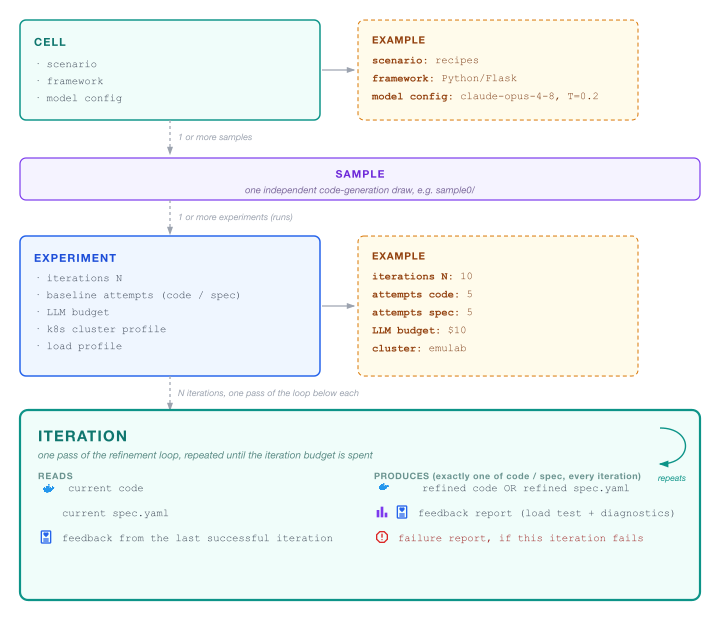
\includegraphics[width=1\linewidth]{figures/methods/sample-experiment-diagram.png}
    \caption{Hierarchy of the four experimental units used throughout this
      thesis: cell, sample, experiment, and iteration.}
    \label{fig:sample-experiment-diagram}
\end{figure}

A \textbf{cell} is one point in our experimental design, defined by a tuple
of the \emph{BaxBench scenario} (the application workload and API contract
to implement), the \emph{framework} (the implementation language and
library stack), and the \emph{language-model configuration} (the model used
to generate the application).

\medskip

A \textbf{sample} is one independent execution trajectory for a given
cell. Because LLM behaviour is stochastic, repeated samples of the same
cell allow us to observe independent trajectories, estimate variance, and
obtain a clearer signal about the underlying mean performance of that
cell.

\medskip

An \textbf{experiment} defines the execution and evaluation settings for a
sample:
\begin{itemize}
  \item the number of refinement iterations~$N$;
  \item maximum baseline attempts for code generation and
        deployment-specification generation;
  \item an optional LLM spend cap;
  \item the cluster profile (available hardware and system configuration)
        and the load-test profile (Section~\ref{sec:methods-bench}), plus
        related deploy/bench timeouts.
\end{itemize}
LLM expenditure is also tracked at the experiment level. This supports
budgeting and cost-aware comparison across models
(Section~\ref{sec:methods-metrics}).

\medskip

An \textbf{iteration} is one pass through the refinement pipeline, executed
within a single experiment. It takes the current application state (the
current code and deployment specification) together with the previous
iteration's outcome: either a feedback report summarising load-test results
and system-utilisation diagnostics, or a failure report from an
unsuccessful iteration. It then refines
\emph{exactly one} of the two, either the application code or the
deployment specification. Successful iterations produce a feedback report;
failed iterations produce a failure report.

Having introduced this hierarchy, we now turn to the internal structure of a
single iteration: the sequence of stages that constitute the refinement loop
shown in Figure~\ref{fig:pipeline}.

\FloatBarrier

\subsection{The Iteration Loop}
\label{sec:methods-loop}

\begin{figure}[htbp]
  \centering
  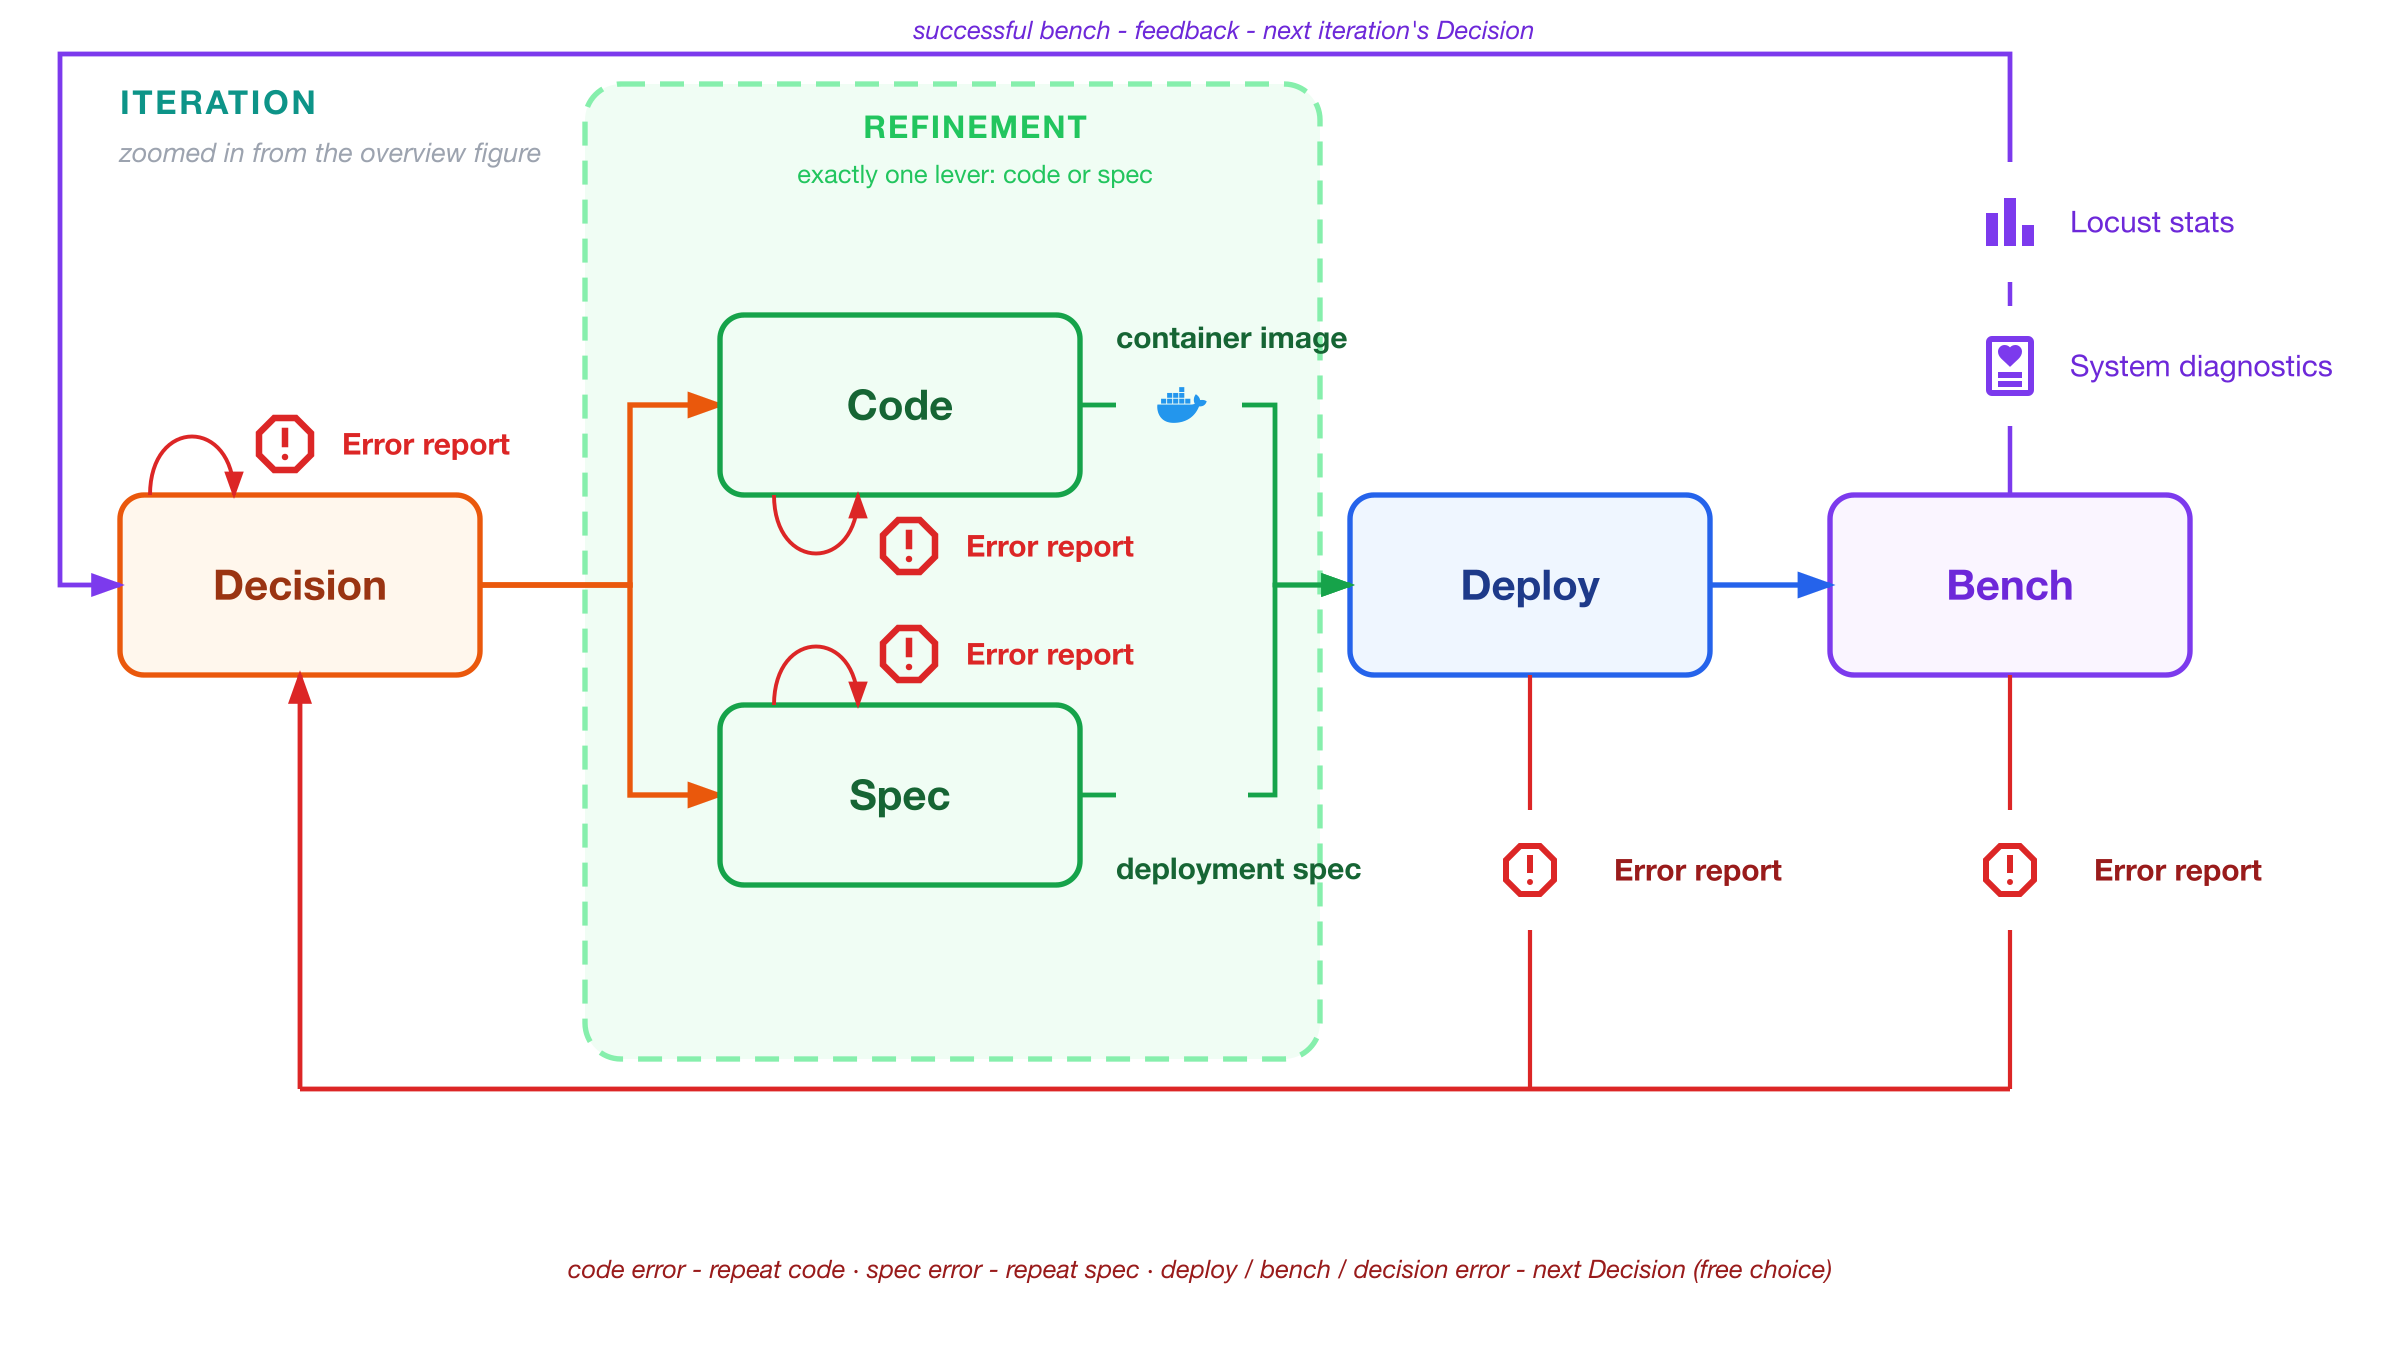
\includegraphics[width=1\linewidth]{figures/methods/iteration-workflow-diagram.png}
  \caption{Refinement-iteration workflow. Each refinement iteration
    progresses through a fixed sequence of decision, refinement,
    deployment, and benchmarking stages.}
  \label{fig:pipeline}
\end{figure}

Every refinement iteration of an experiment follows the same stage order
(Figure~\ref{fig:pipeline}). The baseline iteration differs because it must
generate both optimisation artifacts and is explained separately in
Section~\ref{sec:methods-baseline-refinement}.
The stages have fixed responsibilities:

\paragraph{Decision.}
Given any available prior outcome context --- either a feedback report
summarising load-test results and system-utilisation diagnostics, or a
failure report --- the agent selects a refinement action: either refine the
\textbf{application code} or refine the \textbf{deployment specification}.

\paragraph{Code.}
If the agent decides to refine the application, it is prompted to generate
updated application code. That code must pass the scenario's functional
tests; upon passing, the application is built into a container image for
later deployment.

\paragraph{Spec.}
If the agent decides to refine the deployment configuration, it generates an
updated deployment specification describing the desired Kubernetes
deployment. The specification is then statically validated before
deployment.

\paragraph{Deploy.}
The latest deployment specification is combined with the backend container
image to render Kubernetes manifests, which are then applied
within a newly created namespace. The framework then waits until the
deployment reaches a ready state and all required service endpoints become
available.

\paragraph{Bench.}
Once the deployment is ready, the framework executes a distributed load test
against the application, collecting load-test results and
system-utilisation diagnostics during execution. After a successful run, the
framework summarises them into an iteration feedback report that serves as
input for the next iteration (Section~\ref{sec:methods-outcome}).

\medskip

In refinement iterations, code regeneration and deployment-specification
regeneration are mutually exclusive: exactly one of the two artifacts is
regenerated per iteration, while the other is reused unchanged from the most
recent iteration that produced it (Section~\ref{sec:methods-artifacts}).
This choice improves attribution, since an observed performance change can
be associated with either an application or a deployment-specification
change, and reduces LLM cost, since each refinement iteration requires only
a single regeneration step. It assumes that iteration feedback typically
points towards either an application-level or a deployment-level
bottleneck, making it sufficient to refine one artifact at a time. The
decision stage (or a forced retry after failure;
Section~\ref{sec:methods-failure}) selects which refinement path to follow.

\FloatBarrier

\subsection{Artifact Lineage}
\label{sec:methods-artifacts}

An experiment is \textbf{stateful across iterations} through reusable
artifacts, outcome reports, and the agent's conversation history.

\textbf{Reusable cross-iteration artifacts.} The Code stage produces the
current application state, and the Spec stage produces the current
deployment specification. In each refinement iteration, exactly one of
these two optimisation artifacts is regenerated while the other is carried
forward unchanged from the previous validated lineage. Figure~\ref{fig:artifact-lineage}
traces this carry-forward and shows how failures determine which artifact
versions remain in use.

\textbf{Decision context.} Bench, on success, produces the feedback report
summarising load-test results and system-utilisation diagnostics for the
next Decision. Any stage, on failure, instead produces a failure report.
These reports are used only by the subsequent decision rather than being
continually carried forward as lineage state. After a Code or Spec failure,
the report forces an immediate retry of the same lever and supplies the
specific failure to the subsequent Code or Spec stage. After a Deploy or
Bench failure, it is returned to Decision as free-choice context
(Section~\ref{sec:methods-failure}).

The routing in Figure~\ref{fig:artifact-lineage} keeps invalid Code or Spec
outputs out of the reusable lineage. By contrast, a Deploy or Bench failure
does not by itself identify either artifact as invalid, so the latest
validated versions remain available while the failure report returns to
Decision.

\begin{figure}[htbp]
  \centering
  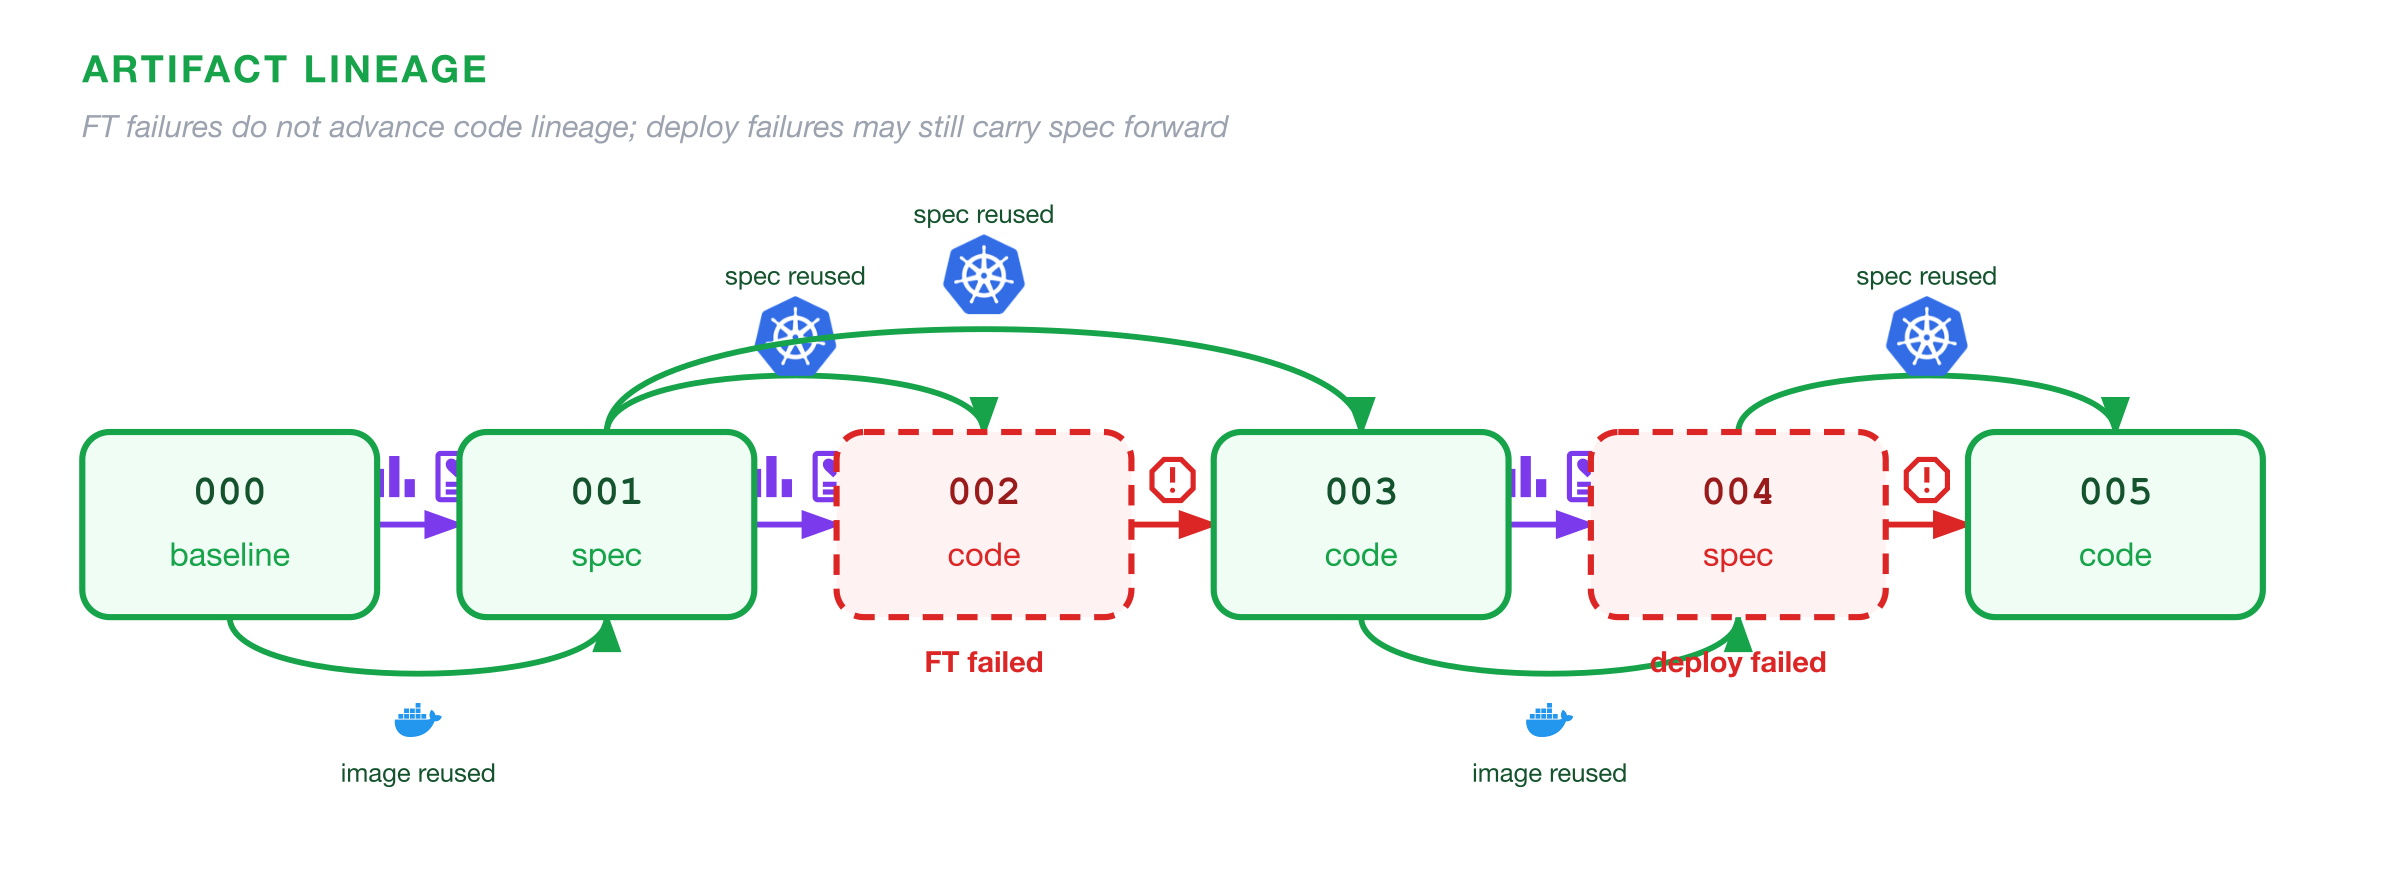
\includegraphics[width=1\linewidth]{figures/methods/artifact-lineage-diagram.png}
  \caption{Example artifact lineage through six iterations. Iteration 001
    refines the deployment specification while reusing the baseline image.
    The failed code refinement in 002 does not advance code lineage and
    forces the successful code retry in 003, with the specification from
    001 carried across both iterations. The specification produced in 004
    remains available after deployment fails; Decision then selects code
    refinement in 005, which reuses that specification and the image from
    003.}
  \label{fig:artifact-lineage}
\end{figure}

\textbf{Iteration-local execution state.} Furthermore, outputs from one
stage become inputs to later stages within an iteration. Deploy combines
the artifact regenerated in that iteration with the artifact carried
forward from the validated lineage to create a running deployment. It then
hands Bench a deployment record containing the namespace, resolved target,
and port, which Bench uses to target the service under test.

\paragraph{Conversation history as agent context.}
The structured lineage above is how the framework carries state across
iterations. The agent itself also has access to prior work through the
conversational thread of the experiment described in
Section~\ref{sec:methods-memory}: later prompts can refer back to earlier
\texttt{<CODE>} and \texttt{<SPEC>} proposals rather than reintroducing
them from scratch. Lineage determines which artifacts the framework carries
forward for execution, while the conversation thread gives the agent access
to its earlier proposals, decisions, and feedback.

\subsection{Responsibility Split}
\label{sec:methods-responsibility}

The LLM agent and the framework have a fixed division of responsibilities,
summarised in Table~\ref{tab:responsibility-split}. The agent decides which
lever to refine and proposes either application code or a deployment
specification. The framework validates these proposals, enforces cluster
constraints, and handles their execution through deployment, benchmarking,
and measurement. The agent therefore reasons about application and deployment
changes without editing raw Kubernetes manifests or executing commands on
cluster nodes. This bounds its search space and separates optimisation
\emph{reasoning} from infrastructure \emph{syntax and execution}.

\begin{table}[htbp]
  \centering
  \caption{Responsibility split by iteration stage.}
  \label{tab:responsibility-split}
  \small
  \renewcommand{\arraystretch}{1.16}
  \setlength{\tabcolsep}{7pt}
  \begin{tabularx}{\linewidth}{@{}>{\raggedright\arraybackslash}p{0.12\linewidth}
      >{\raggedright\arraybackslash}X
      >{\raggedright\arraybackslash}X@{}}
    \toprule
    \textbf{Stage} & \textbf{LLM agent} & \textbf{Framework} \\
    \midrule
    \rowcolor{black!5}
    \textbf{Decision} &
      Decides whether to refine code or deployment &
      Failure routing (Section~\ref{sec:methods-failure}) \\
    \textbf{Code} &
      Proposes application code &
      Functional testing and image build \\
    \rowcolor{black!5}
    \textbf{Spec} &
      Proposes deployment specification &
      Static validation against cluster capacity \\
    \textbf{Deploy} &
      - &
      Manifest rendering, deployment, and readiness checks \\
    \rowcolor{black!5}
    \textbf{Bench} &
      - &
      Benchmarking and utilisation measurement \\
    \bottomrule
  \end{tabularx}
\end{table}

\FloatBarrier

\subsection{Baseline Versus Refinement Iterations}
\label{sec:methods-baseline-refinement}

The workflow differs conceptually between the baseline and later refinement
iterations. Because neither application code nor a deployment specification
exists at iteration~0, both artifacts must be generated and the Decision stage
is skipped. The objective is to produce application code that passes functional
testing and a deployment specification that passes static cluster-capacity
validation, providing validated candidates for execution. This does not
guarantee that deployment or benchmarking will succeed. If either stage fails,
the iteration records a failure report and the experiment proceeds to the next
iteration with that report as context.

\begin{figure}[htbp]
  \centering
  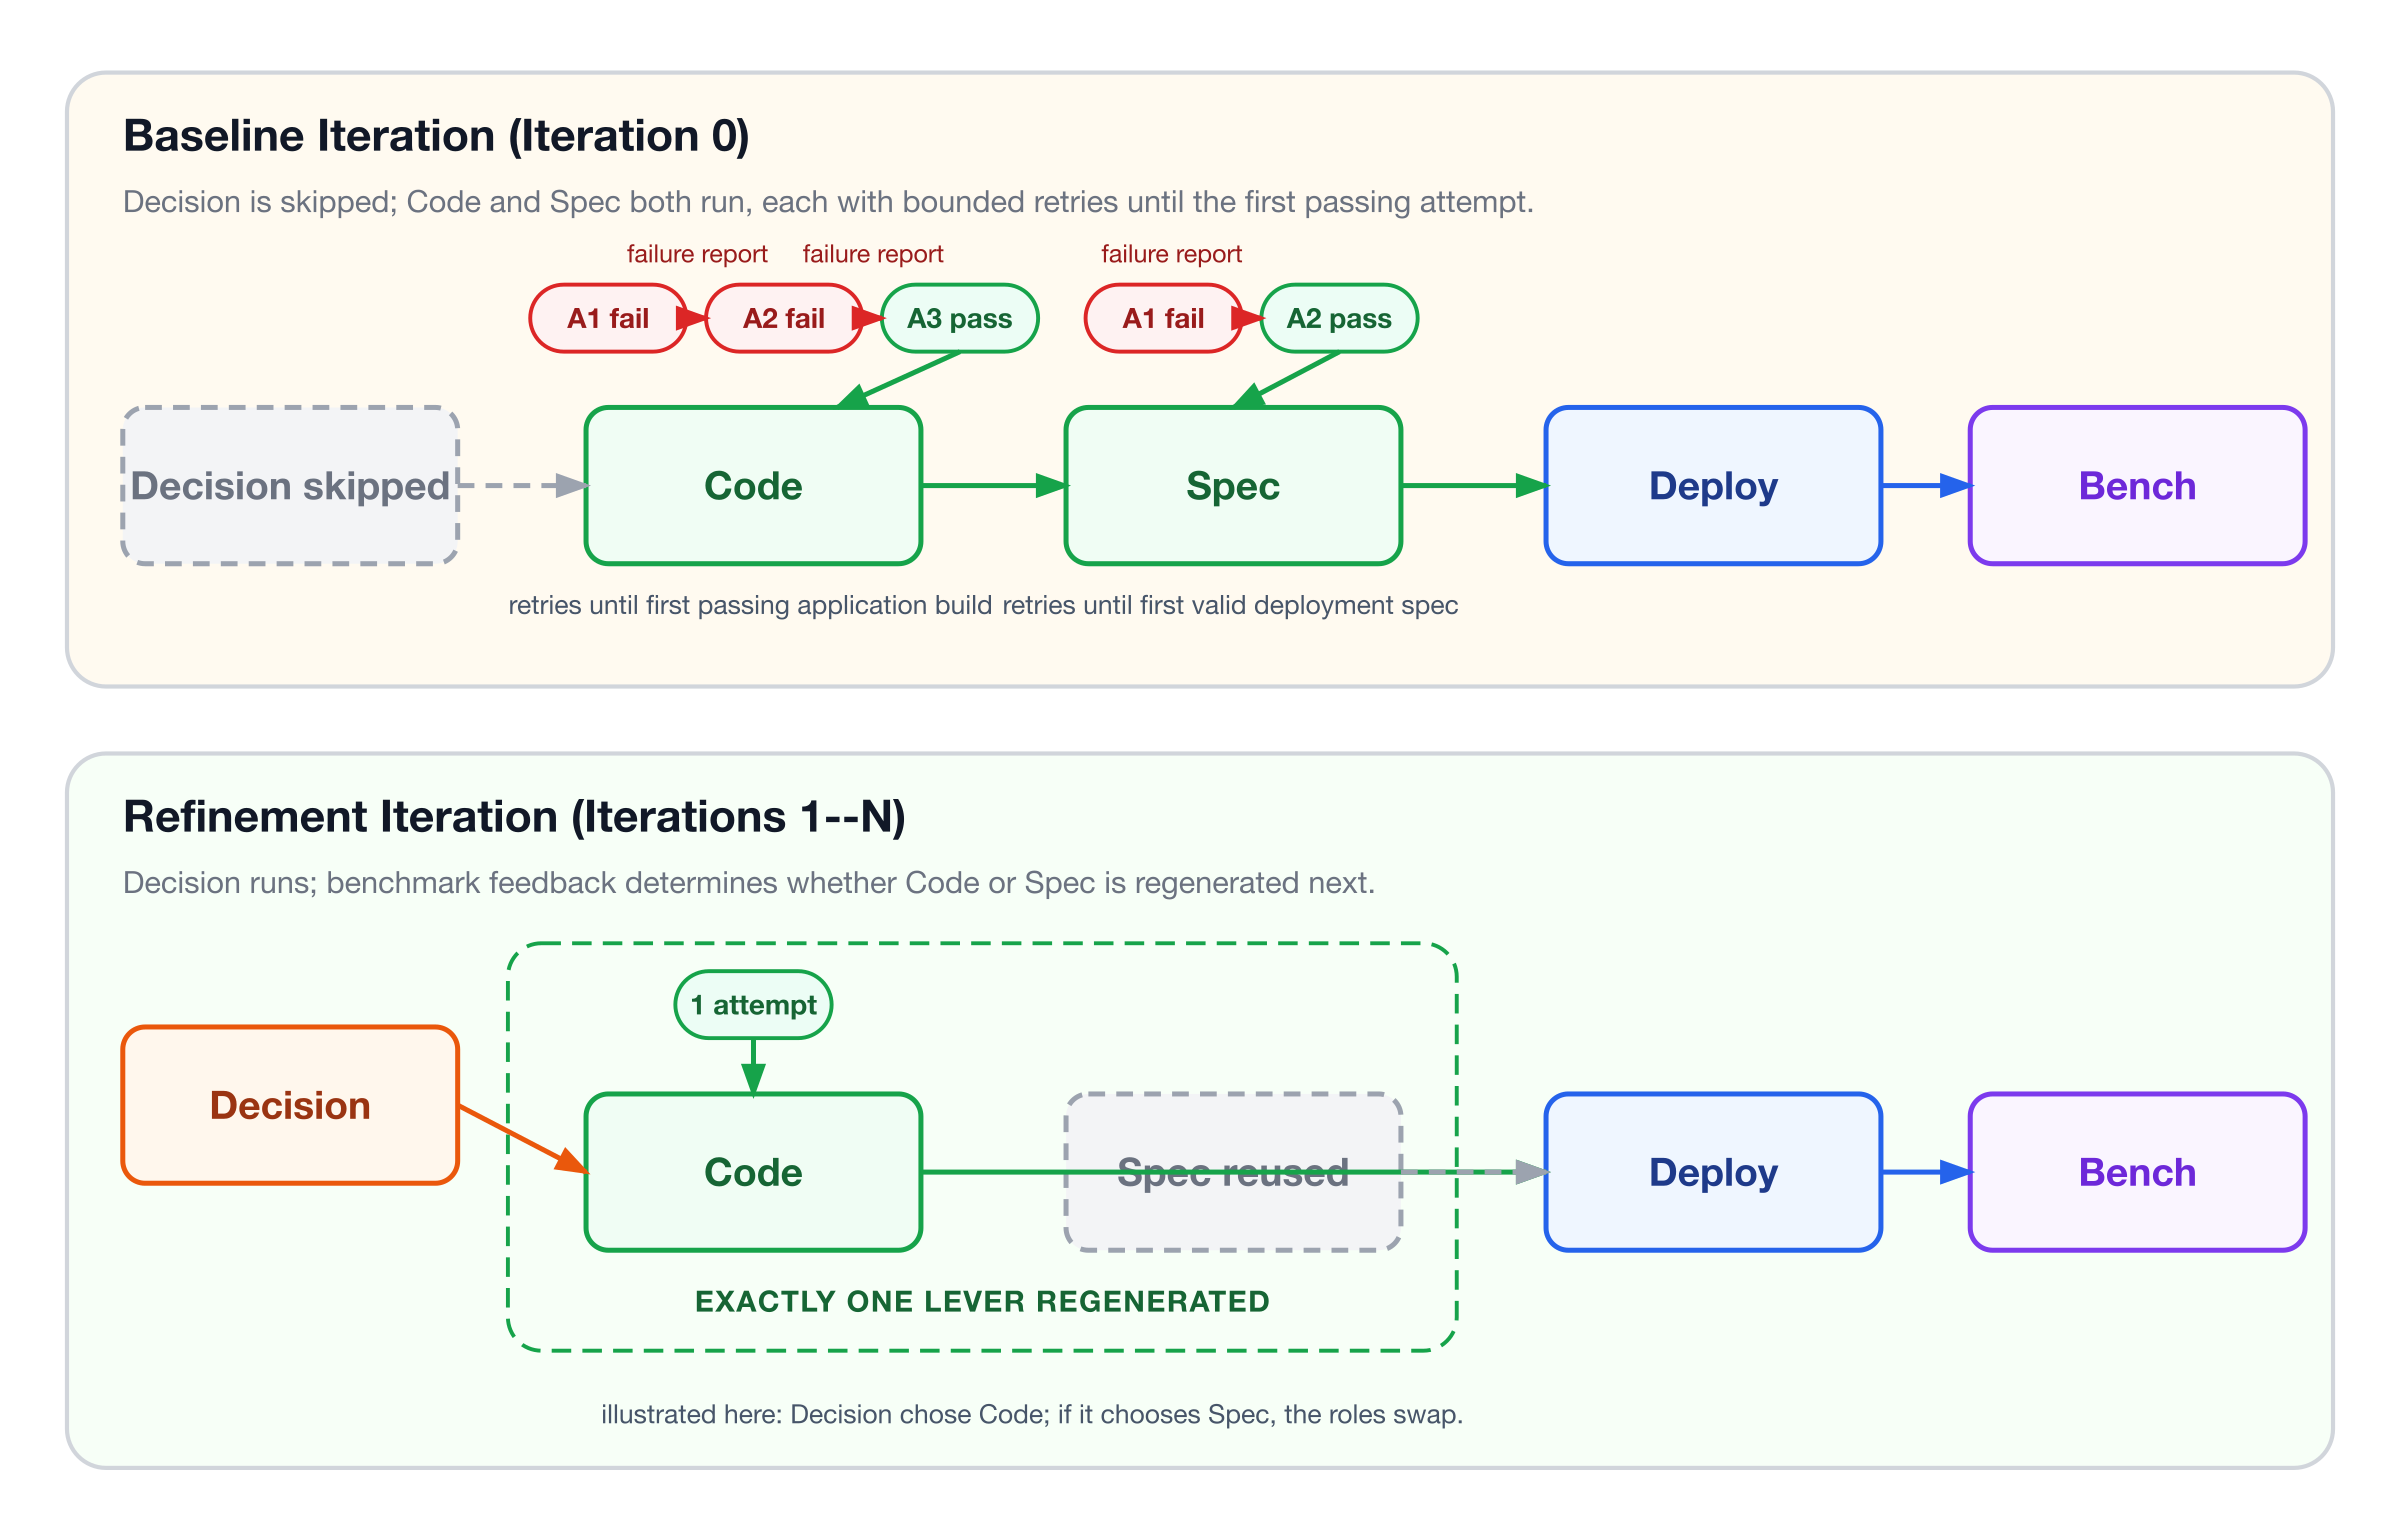
\includegraphics[width=1\linewidth]{figures/methods/baseline-vs-refinement-diagram.png}
  \caption{Baseline and refinement iteration paths. The baseline generates
    both artifacts; subsequent iterations regenerate one and reuse the other.}
  \label{fig:baseline-vs-refinement}
\end{figure}

Baseline generation is intentionally more permissive than later iterations.
Since there is no prior valid artifact to fall back to, code generation and
deployment-specification generation may each be retried when validation fails,
allowing error information from previous attempts to inform subsequent retries.
If no valid baseline can be established within the configured retry budget, the
sample is aborted.

Once a valid code artifact and deployment specification exist, subsequent
iterations follow the general refinement loop described above: benchmark
feedback from the latest outcome is fed into Decision, which selects what to
improve next while reusing the other artifact.


\subsection{Agent Memory Model}
\label{sec:methods-memory}

Unlike single-shot BaxBench code generation, each Kubernetes experiment
maintains \textbf{its own conversational thread}.  A shared prompting
component accumulates user prompts and assistant replies across all stages
and iterations of an experiment.

Each stage appends a new user turn to the existing conversation rather than
starting from an empty context.  The resulting assistant response is then
added to the same thread.  As the experiment progresses, the model
therefore retains access to its previous code generations,
deployment-specification proposals, decisions, rationales, and feedback
from earlier iterations.  This allows later refinement steps to build upon
prior work instead of repeatedly solving the same problem from scratch.

\paragraph{Prompt caching.}
Maintaining a growing conversation history improves continuity but also
increases token usage.  To make long-running experiments economically
feasible, we utilise the prompt-caching mechanisms provided by the
underlying model providers.  Because each stage extends the existing
conversation by appending new messages while leaving previous content
unchanged, most requests share a large stable prefix with earlier
requests.  This structure is particularly well suited for provider-side
prompt caching.  In practice, cached tokens are billed at a small fraction
of the cost of newly processed tokens, substantially reducing the cost of
long-running refinement trajectories.

\paragraph{Prompt slimming.}
To further limit token growth, prompts follow a \textbf{slimming policy}.
Rather than repeatedly embedding large artifacts such as source code,
deployment specifications, or benchmark outputs, later stages refer to
previously generated artifacts already present in the conversation
history, and the model is instructed to consult the relevant earlier
messages when required.  This preserves access to prior context while
avoiding unnecessary duplication, allowing experiments to maintain longer
conversational histories within practical context and cost limits.


% ----- §3.4  Phases -----
\section{Iteration Stages}
\label{sec:methods-phases}

This section describes each of the five stages in Figure~\ref{fig:pipeline}
in terms of its role in the experimental workflow, rather than its software
implementation.  Each stage has a clear contract: it consumes a validated
predecessor artifact or outcome, either produces the input required by the
next stage or records why that was not possible, and preserves enough
evidence for the subsequent iteration.  Table~\ref{tab:stage-summary}
provides an overview.  The detailed subsections distinguish an expected
experimental result (for example, a low-goodput benchmark) from a stage
failure (for example, an unavailable load generator).  Section~\ref{sec:methods-failure}
then collects the resulting routing rules.  Representative prompts for the
three LLM-driven stages are reproduced in Appendix~\ref{ch:appendix-prompts};
configuration constants are deferred to Appendix~\ref{ch:appendix-config}.

Each stage may succeed or fail.  A failure report identifies the stage and
its specific kind, retains the relevant evidence, and does not replace the
last validated code or specification in the artifact lineage.  At the next
iteration, failures in code or specification production force a repair of
that same artifact; failures later in the workflow are returned as context
for a new, free decision.  This makes failures observable experimental
outcomes without allowing an invalid artifact to silently become the basis
of later comparisons.

\begin{table}[htbp]
  \centering
  \caption{Iteration stages at a glance. Full detail, including every
    failure kind, follows in the subsections below.}
  \label{tab:stage-summary}
  \small
  \begin{tabular}{@{}p{0.08\linewidth}p{0.18\linewidth}p{0.21\linewidth}p{0.18\linewidth}p{0.19\linewidth}@{}}
    \toprule
    \textbf{Stage} & \textbf{Purpose} & \textbf{Key inputs} & \textbf{Key outputs} & \textbf{Failure boundary} \\
    \midrule
    Decision &
      Pick the next refinement lever &
      Prior feedback or failure; conversation history &
      Recorded decision + rationale &
      No usable choice from the agent \\
    Code &
      Produce a container-ready, tested application &
      Scenario spec; prior code turn; prior test failures &
      Docker image + source tree &
      Invalid response, build, or functional-test failure \\
    Spec &
      Produce a validated \texttt{spec.yaml} &
      Cluster capacity; prior spec turn; validation errors &
      \texttt{spec.yaml} &
      Invalid schema or infeasible resource plan \\
    Deploy &
      Bring the candidate up on the cluster &
      \texttt{spec.yaml}; image reference &
      Probe record (namespace, target) &
      Candidate cannot become reachable and ready \\
    Bench &
      Measure sustained goodput under load &
      Probe record; load profile &
      Feedback report &
      Harness/target failure; low goodput is a result, not a failure \\
    \bottomrule
  \end{tabular}
\end{table}


\subsection{Decision Stage}
\label{sec:methods-decision}

\paragraph{Purpose.}
Choose which single artifact, application code or deployment specification,
the rest of this iteration will refine, so as to raise sustained goodput. It
runs for every refinement iteration ($\geq 1$); the baseline
(Section~\ref{sec:methods-workflow}) skips it entirely, since baseline
iteration~0 always regenerates both.

\paragraph{Inputs.}
The agent receives the established conversation context, the current valid
code and specification as references, and one outcome from iteration
$N{-}1$: either benchmark feedback after a completed benchmark or a failure
report when the iteration stopped earlier.  The former is the report defined
in Section~\ref{sec:methods-bench}; it states the measured load behaviour
and diagnostics, rather than merely a scalar score.  The two context types
are mutually exclusive, so the decision is always grounded in the immediate
predecessor's actual outcome.

\paragraph{Processing.}
The workflow first checks whether $N{-}1$ failed, and if so, at which phase:
\begin{itemize}
  \item a \textbf{code} failure forces \textbf{code} again, and a
        \textbf{spec} failure forces \textbf{deployment} again (the
        deterministic routing rules of Section~\ref{sec:methods-failure});
        in both cases the decision LLM is skipped entirely;
  \item a \textbf{decision}, \textbf{deploy}, or \textbf{bench} failure does
        not force a lever, so the LLM is called and chooses freely, with the
        failure block as its context instead of a benchmark summary;
  \item if $N{-}1$ was itself the baseline and it failed, the sample aborts
        before any of the above: there is no working system to refine.
\end{itemize}
When a free choice is permitted, the prompt requires one of the two levers
and a short rationale.  An experiment may alternatively fix the lever as an
ablation.  A malformed response or an unavailable model call is a Decision
failure.  Appendix~\ref{ch:appendix-prompts} gives the corresponding prompt,
including the successful-iteration feedback placeholder.

\paragraph{Outputs.}
The selected lever and rationale determine which artifact is regenerated;
the other remains the last validated version (Section~\ref{sec:methods-artifacts}).

\paragraph{Failure Modes.}
Decision fails only when no usable choice can be obtained, for example after
a model-service failure or a response that does not identify one permitted
lever.  It does not fail because a choice is expected to perform poorly;
that question belongs to Bench.

\paragraph{Feedback.}
On failure, the recorded service error or malformed response becomes context
for the next free decision.  On success, the decision is immediately
consumed by the Code and Spec stages; it introduces no performance claim on
its own.

\paragraph{Why single-lever decisions.}
Deployment tuning and code optimisation are coupled but costly to change
jointly: forcing exactly one lever per iteration keeps attribution clean, an
observed goodput change can be traced to either the application or the
deployment shape, never both at once, at the cost of assuming that a given
round of feedback points predominantly at one or the other.


\subsection{Code Generation and Functional Tests}
\label{sec:methods-code}

\paragraph{Purpose.}
Produce a container-ready, functionally passing application build, or, when
this iteration refines the deployment specification instead, reuse the
current one untouched.

\paragraph{Inputs.}
Baseline generation receives the scenario contract and target framework.
Code refinement additionally receives the current valid code through the
conversation context and, after a previous code failure, the associated
test or build evidence. When the deployment lever was selected, no new
code is generated: the current validated code and image are reused.

\paragraph{Processing.}
\begin{itemize}
  \item \textbf{Baseline:} up to a configured number of attempts
        (Appendix~\ref{ch:appendix-config}). Each attempt calls the LLM,
        parses its \texttt{<FILEPATH>}/\texttt{<CODE>} output into files,
        and runs the scenario's functional-test suite inside a container;
        the loop stops at the first pass. An attempt that fails because the
        test \emph{harness itself} could not start (for example, a Docker or
        Postgres port bind failure) is flagged as infrastructure rather than
        an application bug and aborts the retry loop immediately rather than
        spending further attempts on a problem the agent cannot fix by
        rewriting code.
  \item \textbf{Code refinement:} exactly one attempt, the same
        call/parse/test sequence, fail-fast (no internal retry within the
        iteration).
  \item \textbf{Deployment refinement:} no LLM call. The source tree and its
        already-built image reference are copied verbatim from the lineage
        pointer; the image is not rebuilt, since the code did not change.
\end{itemize}
Functional tests gate every path that can produce a new image; only a
passing build is ever deployed. Example baseline and refinement prompts are
given in Appendix~\ref{ch:appendix-prompts}.

\paragraph{Outputs.}
On success, the stage yields a tested application image and its source
artifact. This is the only kind of newly generated application that may be
deployed.

\paragraph{Failure Modes.}
Classified into kinds that change what the next code (or decision) prompt
emphasises: \textbf{functional-test} failures (one or more scenario tests
fail; the record keeps per-test logs, a coarse failure category such as
timeout versus server error versus wrong response, and the list of tests
still passing, so the next attempt does not regress them); \textbf{build}
failures (the image did not compile; tests never ran); \textbf{infrastructure}
failures (the test harness itself could not start, explicitly labelled as
\emph{not} an application bug); \textbf{LLM call or parse} failures; and
\textbf{test-runner} failures (the functional-test runner process crashed,
independent of any assertion outcome).

\paragraph{Feedback.}
A failed refinement keeps the previous passing code in the lineage and
forces the next iteration to repair code with the recorded evidence
(Section~\ref{sec:methods-failure}). If baseline attempts are exhausted,
the sample cannot proceed because it has no functional application.
Successful code becomes Deploy's input; only the later benchmark produces
performance feedback.


\subsection{Deployment Specification}
\label{sec:methods-spec}

\paragraph{Purpose.}
Produce \texttt{spec.yaml}, a structured description of the desired
Kubernetes deployment. This stage is central to the thesis's contribution:
the agent never writes Kubernetes manifests directly; it fills in a bounded
schema, and the framework alone turns that schema into manifests (Deploy,
below) so that comparisons stay about deployment \emph{decisions} rather
than YAML-authoring skill.

\paragraph{Inputs.}
The stage receives the cluster's allocatable worker capacity and the
application context.  Deployment refinement additionally refers to the
current valid specification and, after a prior specification failure, its
validation evidence.  During code refinement, the current validated
specification is reused unchanged.

\paragraph{Processing.}
The LLM returns a \texttt{<SPEC>} YAML fragment covering \texttt{backend},
optional \texttt{pooler}/\texttt{read\_pooler}/\texttt{cache}, and
\texttt{database} (Table~\ref{tab:spec-schema}); the framework merges it
onto fields it always controls itself (container image reference,
listening port, namespace, and database connection variables are never
agent-settable), resolves any named node-placement constraints, and runs
static validation against the capacity snapshot above. Baseline gets a
configured number of outer attempts (Appendix~\ref{ch:appendix-config}),
each of which may itself re-prompt the LLM a small number of times to
correct a parse or validation error before that outer attempt is recorded
as failed; refinement gets exactly one outer attempt with no internal
retry, fail-fast, matching the code stage's refinement behaviour. The
prompt documents field semantics, hard scheduling constraints, and a short
list of qualitative diagnostic heuristics (for instance, that idle read
replicas alongside a saturated primary usually mean the application code
never queries the replica); it never suggests a concrete numeric target
such as a replica count or a CPU request, so any specific value in the
resulting spec is the agent's own inference from capacity and prior
feedback, not a value copied from the prompt. An example spec prompt is
given in Appendix~\ref{ch:appendix-prompts}.

Static validation checks, run for every pod type the schema can request
(backend, Postgres primary, Postgres read replicas, both poolers, and both
Redis caches): each pod's resource \emph{requests} fit on at least one
allowed worker; the cluster-wide sum of requests stays within advertised
capacity after a fixed reserve; and, whenever the agent sets
\texttt{backend.env.DB\_POOL\_SIZE} (the check is skipped, with a warning,
if it does not), a connection-budget check whose exact form depends on
whether a pooler is in the spec: without one,
$\text{backend.replicas} \times \text{pool\_size} \leq
\text{database.max\_connections}$ must hold directly against Postgres; with
one, the same client-connection estimate must instead fit the pooler's own
\texttt{max\_client\_conn}, and symmetrically for \texttt{read\_pooler} when
enabled (which additionally requires \texttt{database.replicas}~$>1$).

Static validation is the \emph{only} check this stage performs: it never
applies anything to the cluster. A spec that passes is guaranteed
schedulable on paper, not yet known to actually come up, that is what the
Deploy stage checks next (Section~\ref{sec:methods-deploy}).

\begin{table}[t]
  \centering
  \caption{Deployment specification schema (agent-controlled fields).}
  \label{tab:spec-schema}
  \small
  \begin{tabular}{@{}p{0.35\linewidth}p{0.6\linewidth}@{}}
    \toprule
    \textbf{Field} & \textbf{Effect} \\
    \midrule
    \texttt{backend.replicas} & Horizontal scale behind the backend Service \\
    \texttt{backend.resources.*} & Per-pod CPU/memory request and limit \\
    \texttt{backend.placement.\allowbreak workers}, \texttt{.spread\_replicas} & Node allow-list; anti-affinity across nodes \\
    \texttt{backend.env.*} & Allow-listed runtime knobs the app must itself read, e.g.\ \texttt{DB\_POOL\_SIZE}, \texttt{WEB\_CONCURRENCY}, \texttt{GOMAXPROCS} \\
    \texttt{pooler.*} & Optional PgBouncer in front of the Postgres primary: \texttt{enabled}, \texttt{mode}, \texttt{replicas}, \texttt{max\_client\_conn}, \texttt{default\_pool\_size}, \texttt{resources} \\
    \texttt{read\_pooler.*} & Same fields, in front of read replicas; requires \texttt{database.replicas}~$>1$ \\
    \texttt{cache.*} & Optional application-level Redis: \texttt{enabled}, \texttt{replicas}, \texttt{maxmemory}, \texttt{resources} \\
    \texttt{database.replicas} & $1$ = standalone; $N{>}1$ = 1 primary + $(N{-}1)$ streaming read replicas \\
    \texttt{database.max\_connections} & Postgres primary connection ceiling \\
    \texttt{database.resources.*}, \texttt{.primary.resources}, \texttt{.replica.resources} & Default, and optional asymmetric overrides, per DB role \\
    \texttt{database.placement.\allowbreak worker}, \texttt{.placement.workers} & Pin or restrict DB pod placement \\
    \texttt{database.tuning.*} & 11 Postgres GUCs (memory: \texttt{shared\_buffers}, \texttt{work\_mem}, \ldots; parallelism; checkpoint/WAL; planner cost; statement timeout); full list in Appendix~\ref{ch:appendix-prompts} \\
    \texttt{database.cache.*} & Optional DB-adjacent Redis, shared with \texttt{cache} or dedicated \\
    \bottomrule
  \end{tabular}
\end{table}

\paragraph{Outputs.}
A validated workload plan, together with its capacity assessment and any
warnings.  On the code-refinement path, the prior validated plan is carried
forward without modification.

\paragraph{Failure Modes.}
\textbf{Validation} failures (a capacity, scheduling, or connection-budget
violation; the record keeps the explicit error and warning list) or
\textbf{LLM call/parse} failures.

\paragraph{Feedback.}
A failed refinement attempt is recorded as a spec failure; the next
iteration is \textbf{forced} onto the \textbf{deployment} lever with those
validation errors as context (Section~\ref{sec:methods-failure}). Exhausting
the baseline attempt budget aborts the sample.

\FloatBarrier

\subsection{Deploy and Readiness Probe}
\label{sec:methods-deploy}

\paragraph{Purpose.}
Turn a validated \texttt{spec.yaml} into a running, reachable cluster
deployment, and answer only whether this layout comes up, deliberately
before any load is applied (Table~\ref{tab:deploy-vs-bench}). Deploy always
runs, for baseline and every refinement iteration alike, regardless of
which lever was refined.

\begin{table}[t]
  \centering
  \caption{The two questions Deploy and Bench each answer.}
  \label{tab:deploy-vs-bench}
  \small
  \begin{tabular}{@{}lp{0.62\linewidth}@{}}
    \toprule
    \textbf{Stage} & \textbf{Question answered} \\
    \midrule
    Deploy & Can this layout be scheduled and become ready? \\
    Bench (Locust) & What sustained goodput does it achieve under load? \\
    \bottomrule
  \end{tabular}
\end{table}

\paragraph{Inputs.}
This iteration's validated workload plan and tested application image,
whether newly generated or carried forward, plus framework-owned runtime
settings such as image wiring, service exposure, and experiment isolation.

\paragraph{Processing.}
The framework renders and applies the workload in a fresh, isolated
deployment context; agent-controlled planning fields are kept distinct from
runtime wiring.  It then verifies that each requested workload is ready,
that the backend is reachable through its service, and that required
database services expose endpoints.  Deploy is deliberately a single
attempt in both baseline and refinement iterations: it tests whether this
specific candidate can run, rather than masking a deployment outcome with
unobserved retries.

\paragraph{Outputs.}
A deployment record identifying the reachable backend target and the
resolved runtime configuration. Bench uses this record to test exactly the
candidate that passed readiness.

\paragraph{Failure Modes.}
Heuristically classified from \texttt{kubectl} output and cluster
diagnostics into image-pull errors, unschedulable pods, crash loops,
out-of-memory kills, failing readiness probes, unavailable service
endpoints, manifest-apply errors, namespace-cleanup errors, timeouts, and an
unknown fallback.

\paragraph{Feedback.}
The failure record (category, \texttt{kubectl wait} details, a diagnostics
excerpt) is captured, and the next decision is asked to adjust replicas,
resources, or placement, but deploy failures do \textbf{not} force a lever:
the next decision LLM chooses freely between code and deployment, since a
deployment that fails to come up could plausibly be fixed by a smaller or
differently placed spec, or, less commonly, by an application change (for
example, one that never becomes ready under its configured probe).

\FloatBarrier

\subsection{Load Benchmark}
\label{sec:methods-bench}

\paragraph{Purpose.}
Measure the deployed candidate's maximal sustained goodput under load, and
close the iteration by turning that measurement into the next iteration's
decision context. Bench always runs after a successful deploy, for baseline
and every refinement iteration alike.

\paragraph{Inputs.}
The deploy probe record (namespace, target, port); this iteration's
\texttt{spec.yaml}, read only to configure which diagnostics collectors to
attach (for example, whether a pooler or read replica is present); the
scenario's Locust task definitions, the same API surface exercised by
functional tests; and the experiment's load-profile parameters
(Appendix~\ref{ch:appendix-config}).

\paragraph{Processing.}
A fresh liveness check against the backend Service runs first, since pods
can die in the gap between deploy and bench; then a distributed Locust run
driven by the adaptive controller below, with optional diagnostics
collectors sampling in parallel.

\subsubsection{Adaptive Load Profile}
\label{sec:methods-load-profile}

Fixed request rates require per-application tuning and do not automatically
find the capacity knee. The framework instead uses an adaptive load profile
that searches for sustainable throughput in three phases, \emph{explore},
\emph{recovery}, and \emph{refine}, after an initial health-gated warm-up.

\paragraph{Warm-up.}
The controller holds a fixed initial user count for 30\,s and checks that the
deployment is minimally healthy: active users present, requests observed, and
failure rate below threshold.  If this check fails, the bench stops
immediately and \textbf{sustained goodput is recorded as exactly $0$}, even
though some requests may have been served during the failed window: the run
never reaches the explore phase.  This is the mechanism behind the cells in
Chapter~\ref{ch:results} whose baseline reports $0$\,req/s despite the
deployment technically coming up.

\paragraph{Explore.}
Once warm-up passes, virtual users ramp upward in steps sized at $4\%$ of the
current level (floored at 20 users), spaced by a p95-latency-adaptive
interval so faster deployments are probed more often.  Explore tracks the
best rolling goodput observed so far and stops the ramp when \emph{any} of:
\begin{itemize}
  \item failure rate $> 2\%$;
  \item p95 latency $> 1000$\,ms;
  \item goodput falls below $95\%$ of the best value seen so far for three
        consecutive checks (collapse);
  \item the user ceiling ($100{,}000$) is reached.
\end{itemize}
Explore locates an approximate overload boundary; it is not itself a
measurement of sustainable throughput.

\paragraph{Recovery.}
The controller drops to $75\%$ of the explore-phase peak user count and holds
for 45\,s.  If the deployment is healthy at that level (failure rate and p95
within threshold), recovery hands off to refine.  If not, it drops a further
$15\%$ and re-settles, up to three attempts.  If the deployment is still
unhealthy after the retry budget is exhausted, the bench stops and refine is
never reached: a second, distinct way for a bench to legitimately report
sustained goodput of $0$ (or near-$0$) despite explore having found a
working region earlier in the same run.

\paragraph{Refine.}
From the recovered healthy level, the controller searches upward in
efficiency-scaled steps: each step is the marginal goodput efficiency of the
previous step, times a cap of $5\%$ of the recovery-entry user count, so
steps shrink automatically as the deployment approaches saturation.  A user
level is accepted once ten consecutive 1\,s goodput samples lie within $5\%$
of their mean (stable).  Refine stops as soon as a settled level fails to
beat the previous best (stall), the failure-rate threshold is exceeded, or
the user ceiling is reached, and reports its best accepted level.

\paragraph{Primary metric: goodput.}
\textbf{Goodput} is the sustained rate of \emph{successful} HTTP responses
(requests per second excluding failures).  Raw throughput at high error rates
is not treated as improvement; spec and code prompts align the agent with
goodput maximisation.

\paragraph{Iteration score.}
Two related quantities are reported: \textbf{peak step goodput}, the
maximum per-step goodput observed anywhere in the run across explore,
recovery, and refine steps (useful for adaptive-ramp plots), and
\textbf{sustained goodput}, the best settled refine-phase level, which is
the primary cross-iteration comparison metric. A bench that never reaches
refine, because warm-up or recovery failed its health check, reports
sustained goodput $=0$.
The profile enforces a maximum run time of $1800$\,s ($30$\,min) and a user
ceiling of $100{,}000$; full parameter values are given in
Appendix~\ref{ch:appendix-config}.

\subsubsection{Diagnostics}

Bench collects two complementary kinds of evidence.  First, Locust records
the adaptive-ramp events and an endpoint-level request table: request and
failure counts, failure percentage, median, mean, minimum, maximum, p95 and
p99 latency, request rate, and failure rate.  Its HTTP-error
excerpt preserves the client-visible symptoms.  Second, run-scoped cluster
diagnostics collect application and database log excerpts; pod health and
cluster events; pod and node CPU and memory observations; PostgreSQL
connection, transaction, and activity-state statistics; and, when enabled,
replication, PgBouncer, and cache statistics.

The report is produced deterministically from these recorded files, not by
an additional model call.  It first converts the adaptive-controller log
into a short warm-up/explore/recovery/refine narrative, including stopping
reason, peak step, and accepted sustained level.  It then renders the
Locust endpoint table and error excerpt.  Finally, it groups periodic
diagnostic samples by the relevant component (and, for resource data, by
tier, pod, and node).  Bursty numeric series are reduced to
\emph{minimum / median / arithmetic mean / p95 / maximum}; counters such as
deadlocks and rollbacks are reported as their run-level change.  This
preserves both typical and near-worst-case pressure without placing raw
per-second telemetry in the decision prompt.

The resulting feedback therefore presents, in a stable order, the load-run
summary, endpoint-level Locust statistics, HTTP errors, log and health
signals, database/pooler/cache/replication diagnostics where applicable,
cluster events, and Kubernetes utilisation.  It may also add a derived
cross-component note when the evidence supports it---for example, that read
replicas were idle while the primary was busy.  Missing or disabled
collectors are explicitly marked unavailable rather than interpreted as
healthy.

\paragraph{Outputs.}
On any completed run, whatever goodput value it measured, including exactly
$0$, an iteration-feedback report containing the deterministic summary
above.  It is persisted in both structured and human-readable form so that
the next Decision can inspect the same evidence that supports the result
tables, while the complete raw run remains available for audit.

\paragraph{Failure Modes.}
A completed load test that simply reports low goodput, including exactly
$0$, is a \emph{successful} bench outcome for orchestration purposes: its
score and diagnostics become the prior feedback for a free decision.
Sustained goodput of $0$ specifically arises when the run stops during
warm-up or recovery before ever reaching refine
(Section~\ref{sec:methods-load-profile}); this is distinct from a genuine,
harness-level \textbf{bench failure}, which is one of: a Locust
infrastructure crash (master, worker, or generator), a target-unreachable
error (DNS, connection refused, or timeout to the service), a timeout or
stall, or an unknown fallback.

\paragraph{Feedback.}
\label{sec:methods-outcome}
On a harness failure, the failure record (summary plus a harness log
excerpt) is captured, and, as with deploy failures, the next decision
chooses freely between code and deployment. On success, the feedback report
above becomes the input to the next Decision (Section~\ref{sec:methods-decision})
and, because it is the newest successful outcome, advances the ``latest
good'' lineage pointer for whichever artifact this iteration touched
(Section~\ref{sec:methods-artifacts}). Only successful iterations advance
lineage; a failed iteration's record is retained on disk for audit, but its
structured failure, not a feedback report, is what becomes the next
iteration's context.


% ----- §3.5  Failure routing (summary) -----
\section{Failure Routing Summary}
\label{sec:methods-failure}

Every failure mode in Section~\ref{sec:methods-phases} follows the same
shape: a \textbf{trigger} (what went wrong), \textbf{detection} (how the
framework recognises it, from an explicit non-zero exit code to a heuristic
match against log or diagnostic text), \textbf{captured information} (a
structured failure record persisted to that phase's \texttt{failure.json},
with the specific evidence, e.g.\ failing-test logs, \texttt{kubectl} wait
output, or a Locust error excerpt), and \textbf{agent feedback} (that
record's prompt-formatted block, injected into the next relevant LLM call,
typically the next Decision stage unless the routing rule forces an
immediate retry of the same lever).
The stage subsections above already give the first three for every kind;
this section collects only the fourth: which lever, if any, the next
iteration is routed onto as a result.

Table~\ref{tab:failure-routing} summarises the routing rule for every
failure kind. Two patterns recur. First, a failure in the stage that
\emph{produces} an artifact forces an immediate retry of that same lever: a
code failure forces code, a spec failure forces deployment (deployment
refinement's folder label is \texttt{-spec}, since it is the artifact that
was regenerated), so the agent's very next move is a fix attempt with the
failure detail fresh in context, rather than a free choice that might drift
to the unrelated lever. Second, a failure \emph{downstream} of artifact
production, at decision, deploy, or bench, does not force a lever: the next
decision LLM chooses freely, since the cause could plausibly lie on either
side (a deploy failure might call for a smaller spec, or, less commonly, an
application fix; a bench failure is a harness problem unrelated to either
artifact).

\begin{table}[t]
  \centering
  \caption{Iteration routing after failure.}
  \label{tab:failure-routing}
  \small
  \begin{tabular}{@{}ll@{}}
    \toprule
    \textbf{Failed stage} & \textbf{Next iteration} \\
    \midrule
    Decision & LLM decides freely (with decision failure context) \\
    Code (baseline) & Sample abort (after max attempts) \\
    Code (refinement) & Force \textbf{code} \\
    Spec (baseline) & Sample abort (after max attempts) \\
    Spec (refinement) & Force \textbf{deployment} \\
    Deploy & LLM decides freely \\
    Bench (harness failure) & LLM decides freely \\
    \bottomrule
  \end{tabular}
\end{table}

\FloatBarrier

% ----- §3.6  Design principles -----
\section{Design Principles and Constraints}
\label{sec:methods-design}

\paragraph{Bounded search space.}
Raw Kubernetes YAML is vast and error-prone.  Restricting the agent to a
structured deployment specification keeps comparisons focused on deployment
\emph{decisions} rather than syntactic accidents.

\paragraph{Framework owns infrastructure.}
Network wiring, namespace lifecycle, manifest rendering, Locust orchestration,
and validation rules are fixed.  The agent never executes shell commands on
cluster nodes.

\paragraph{Correctness before performance.}
Functional tests gate all new images; deploy probes gate specs; goodput is
measured only on correct, ready deployments.

\subsection{Cross-Cutting Scenario-Builder Design}
\label{sec:methods-scenario-design}

\paragraph{Conversational context, stable prefixes, and prompt slimming.}
Where an agent is revising an artifact it previously created, it receives an
append-only conversation rather than a fresh prompt. The initial turn carries
the stable scenario or artifact context; later turns add only the outcome or
failure that motivates a revision. Large artifacts already available in the
conversation are referenced rather than repeated. For independent judges, we
instead use fresh decisions with the same stable context prefix and a small,
case-specific suffix. This preserves independent judgments while allowing
provider-side prompt caching to reuse the common prefix. In the provider
configurations used here, cached input is typically charged at roughly one
tenth of the ordinary input-token rate, so this structure materially reduces
the cost of repeated generation and review.

\paragraph{Typed failures and validated artifact progression.}
Every repairable failure is represented as a structured record that states
what failed, the evidence observed, and which agent or component can act on
it. The record is persisted for audit and rendered as concise feedback for the
next relevant attempt. The framework distinguishes an author-repairable
artifact failure from a reference-implementation or infrastructure failure so
that an agent is not asked to repair the wrong object. Provisional candidates
do not become benchmark inputs merely because they were generated: they
advance only after the validation appropriate to their stage has succeeded.
This generalises the failure-routing discipline of
Section~\ref{sec:methods-failure} to the scenario-building process.

\paragraph{Learn from feedback, not from hand-tuned ranges.}
Spec prompts omit recommended numeric values, supporting claims about autonomous
deployment optimisation from measured signals.

\paragraph{Fail-fast refinement, generous baseline.}
Baseline retries bootstrap a working system; single-attempt refinement preserves
a fixed iteration budget and clear per-iteration attribution.

\paragraph{Reproducibility.}
Every LLM call is logged; each iteration is a self-contained experiment
record; cluster topology is codified in a single configuration module rather
than ad-hoc host strings in prompts.


% ----- §3.7  Metrics -----
\section{Metrics and Evaluation Criteria}
\label{sec:methods-metrics}

\paragraph{Primary metric.}
\textbf{Sustained goodput} (successful RPS under the adaptive profile), compared
across iterations and scenarios.

\paragraph{Secondary metrics.}
\begin{itemize}
  \item p50 and p95 latency per endpoint;
  \item failure rate during benchmark;
  \item peak step goodput and adaptive-ramp trajectory;
  \item CPU and memory utilisation from \texttt{kubectl top};
  \item deployment-specification parameters (replicas, requests, placement);
  \item iteration outcome labels and agent decision rationales;
  \item estimated LLM cost per experiment.
\end{itemize}

\paragraph{Sample size and statistical treatment.}
Repeated sampling of the same cell (Section~\ref{sec:methods-workflow}) is
useful in principle for estimating generation variance, but the cost of a
full $N$-iteration refinement trajectory makes it impractical to repeat
across every cell within the available budget: each scenario$\times$framework
cell in this thesis is therefore run as a single sample. Comparisons across
cells, models, and frameworks in Chapter~\ref{ch:results} are consequently
\emph{descriptive}---medians and individual data points, not
significance-tested differences---and should be read as indicative of
direction and magnitude rather than as statistically established effects.

\paragraph{Baselines and ablations (Results chapter).}
Examples for comparison:
\begin{itemize}
  \item baseline deployment only (iteration~0 goodput, no refinement);
  \item forced deployment-only vs.\ code-only vs.\ free (agent-chosen)
        refinement lever;
  \item single-shot deploy without iterative feedback.
\end{itemize}


% ----- §3.8  Implementation -----
\section{Implementation Summary}
\label{sec:methods-implementation}

The evaluation harness is implemented as an extension to BaxBench, adding
three components around the single-shot codegen pipeline: an orchestration
layer that drives the iteration pipeline, validates deployment
specifications, and records failures; a distributed load-generation layer
built on Locust; and a diagnostics layer that collects telemetry during
benchmarking.

Detailed module-level documentation, parameter tables, and prompt templates
are deferred to the appendix and repository documentation to keep this
chapter focused on experimental methodology.
